\documentclass{article}
\usepackage{graphicx} % Required for inserting images
\usepackage[margin=1in]{geometry} % Standard 1-inch margins
\usepackage[colorlinks=true, linkcolor=blue, urlcolor=blue]{hyperref} % Hyperlinks in blue
\usepackage{minted}


\title{\textbf{NBC Rating War: \\The Office vs. Parks and Recreation}}
\author{Fall 2023 \\ CSCI 403  Final Project}
\date{\textbf{Group 2:} \\ Katie Bruce, Rachel Castro, Hanuman Chu, \\Thomas Coates, Allison Pelton}

\begin{document}

\maketitle

\begin{center}
    
\includegraphics[width=0.5\textwidth]{Mines Stacked_1Color-blue.png}
\end{center}

\newpage

\section*{\underline{What is interesting about these datasets?}}
The two datasets used in this project are “The Office Dataset” and “Parks and Recreation Episode Data”. The first dataset concerns the NBC sitcom The Office [1], which aired 201 episodes over nine seasons from 2005 to 2013. The second dataset contains data on the 2009–2015 sitcom Parks and Recreation, which aired 126 episodes and has been compared stylistically to The Office. Though the datasets were published by different users to Kaggle and the data were sourced from different locations, the data are presented in comma-separated values format with columns using the same naming scheme [1] [2]. Each dataset consists of two tables: one containing episode and season numbers, titles, writers, directors, air dates, and viewer numbers and one containing IMDb ratings, vote counts, and episode synopses. There was one exception: production codes were only present in the dataset for The Office. Both datasets were released into the public domain. \\


\section*{\underline{Where was the data obtained?}}
The data was obtained by different users on Kaggle.\\
\begin{enumerate}
    \item B. Cruise,  \href{https://www.kaggle.com/datasets/bcruise/parks-and-recreation-episode-data}{Parks and Recreation Dataset}, Kaggle.com
    
    \item N. Prabhavalkar,\href{https://www.kaggle.com/datasets/nehaprabhavalkar/the-office-dataset}{The Office Dataset}, Kaggle.com.
\end{enumerate}

\section*{\underline{License restrictions}}
 Both data sets are \href{https://creativecommons.org/publicdomain/zero/1.0/}{CC0: Public Domain}. The following is quoted from creativecommons.org: "The person who associated a work with this deed has dedicated the work to the public domain by waiving all of his or her rights to the work worldwide under copyright law, including all related and neighboring rights, to the extent allowed by law. You can copy, modify, distribute and perform the work, even for commercial purposes, all without asking permission."

\section*{\underline{Significant attributes as loaded into the database}}

\begin{figure}[h]
\centering
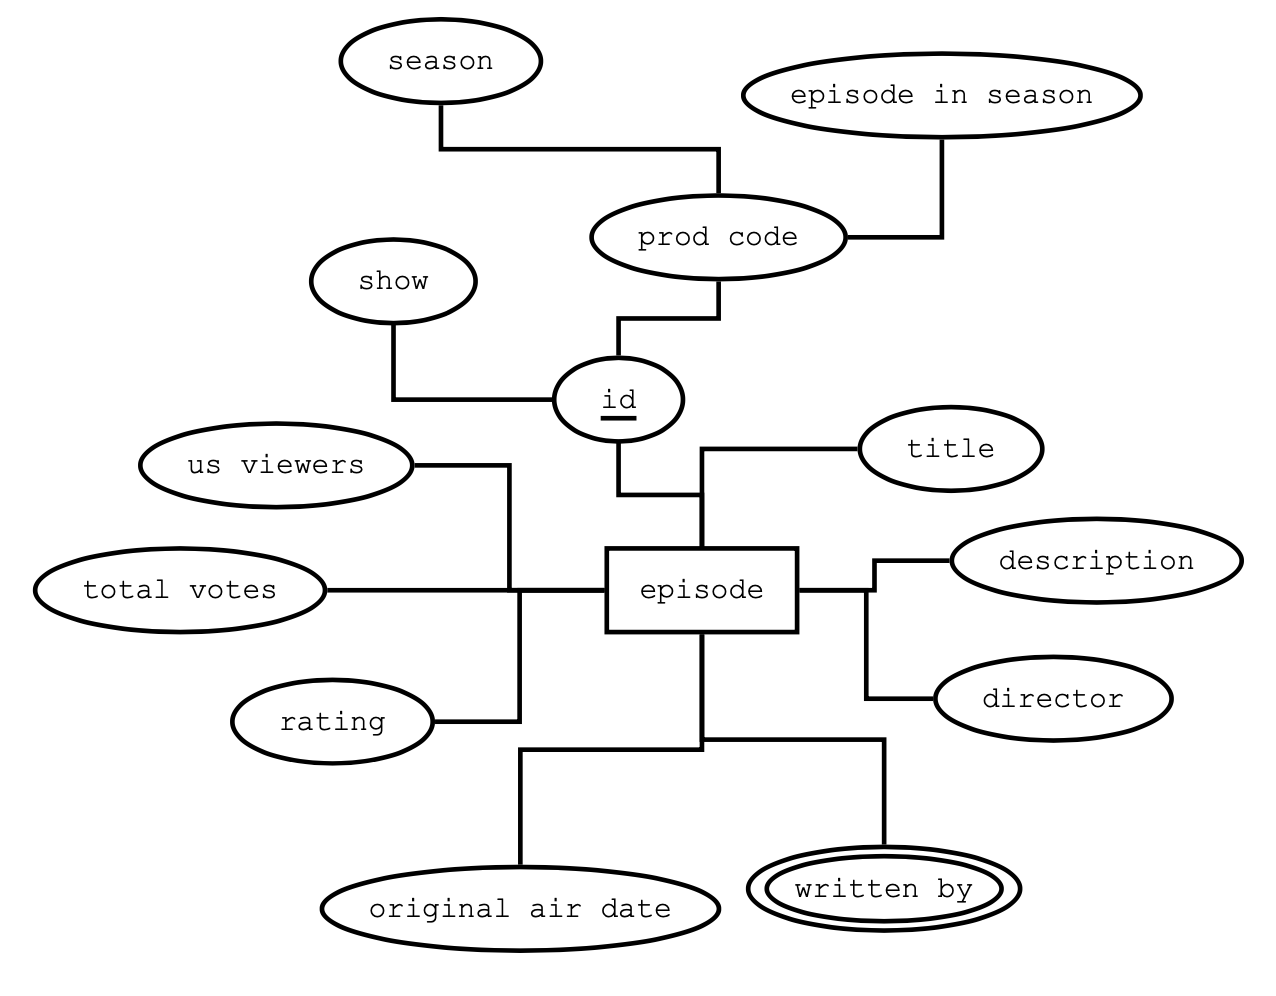
\includegraphics[width=0.5\textwidth]{csci403_final_ER}
\caption{ER diagram}
\label{fig:yourlabel}
\end{figure}

\section*{\underline{Analysis of our datasets}}
\textbf{Functional dependencies:}
\begin{minted}[breaklines]{text}
episode_id -> season, episode_in_season, episode_overall, title, director, writer, air_date, us_viewers, rating, total_votes, description 

episode_overall, show -> episode_id 

show, season, episode_in_season -> episode_overall 

season, episode_in_season -> prod_code 
\end{minted}
Our dataset is normalized to BCNF which you can see by the fact the only functional dependency we have has the superkey of the relation as the functional determiner. 

\section*{\underline{Data loading}}
The attached Python program uses transactions to ensure no data is added anywhere if a single table has errors. Every individual operation is committed only if all table(s) are able to be modified appropriately. 

\section*{\underline{Data Cleaning Operations we Performed}}
The two tables in each dataset contained several duplicate columns, namely season and episode numbers, title, and air date. We determined that an episode can be uniquely identified by its season and episode number, so data were loaded with a uniqueness constraint on those columns in both tables. One may expect an episode title to be unique within a series, but this turned out not to be the case for Parks and Recreation: both S2$\_$E16 and S6$\_$E17 are titled “Galentine’s Day”. 
Due to the limitations of the tool used to load the data files into the database, we loaded the raw data into tables with columns with one-to-one correspondence. To perform data manipulations, the data were inserted into new tables with new formatting using INSERT INTO … SELECT statements. These new tables contained the episode$\_$id column, which was set to the primary key, and converted viewer counts from a float to an int. 
In the raw data, the writers column is a multi-valued attribute. To normalize the dataset, a third table was created containing episode$\_$writer pairs. This was accomplished using the PostgreSQL function regexp$\_$split$\_$to$\_$table() by pattern matching the word “and” and ampersands. 
These cleaning operations result in a database that has no duplicate nor orphaned rating entries. No data is duplicated between tables. Episodes can be added as long as they have a season and episode number provided. 

\section*{\underline{Data growth estimate over the next 10 years}}
\textbf{Current sizes:} \\
\hspace*{1cm} The Office dataset = 52.49 kB\\
\hspace*{1cm} Parks and Recreation dataset = 37.64 kB\\
\textbf{Growth:}\\
\hspace*{1cm} The datasets will likely not grow over time as both the Office and Parks and Recreation finished 
\hspace*{1cm} making new episodes.

\section*{\underline{SQL Security concerns}}
\textbf{Permissions:}
\begin{quote}  
To ensure no unneeded access occurred to the data, we only granted permission to our group members who we trust. Permissions were granted for each group member for each table created and based on group permissions given by the professors, only the trusted group members had access to read, write, and query this database.  
\end{quote}

\textbf{SQL Injection:}
\begin{quote}  
We used /copy to load the dataset so there was no danger of SQL injection because the command only loads data and will not execute any SQL statements. Only our team members are in the project schema group role, preventing unnecessary access to our data. 
\end{quote}


\section*{\underline{Interesting queries done with our data}}

\begin{enumerate}
   
    \item What are the most common words used in the episode descriptions for 'The Office' and 'Parks and Recreation'?"
    \begin{minted}[breaklines]{sql}
    SELECT word, COUNT(*) AS word_count FROM ( 
        SELECT regexp_split_to_table(description, E'\\s+') AS word 
        FROM episode 
        WHERE description IS NOT NULL 
        ) AS words 
        WHERE word NOT IN ('the', 'and', 'is', 'in', 'of', 'it', 'to', 'a', 'for', 'with', 'on', 'as', 'at', 'by', 'an', 'from', 'but', 'or', 'was', 'were', 'are', 'you', 'we', 'they', 'he', 'she', 'it', 'that', 'this', 'his', 'her', 'its', 'their', 'our', 'be', 'have', 'has', 'do', 'did', 'does', 'not', 'what', 'when', 'where', 'how', 'why', 'who', 'which', 'there', 'then', 'if', 'else', 'for', 'while', 'when', 'about', 'into', 'out', 'up', 'down', 'over', 'under', 'between', 'through', 'after', 'before', 'during', 'with', 'without', 'within', 'among', 'between') 
        GROUP BY word 
        ORDER BY word_count DESC 
        LIMIT 20;      
    \end{minted}
    \begin{center}     
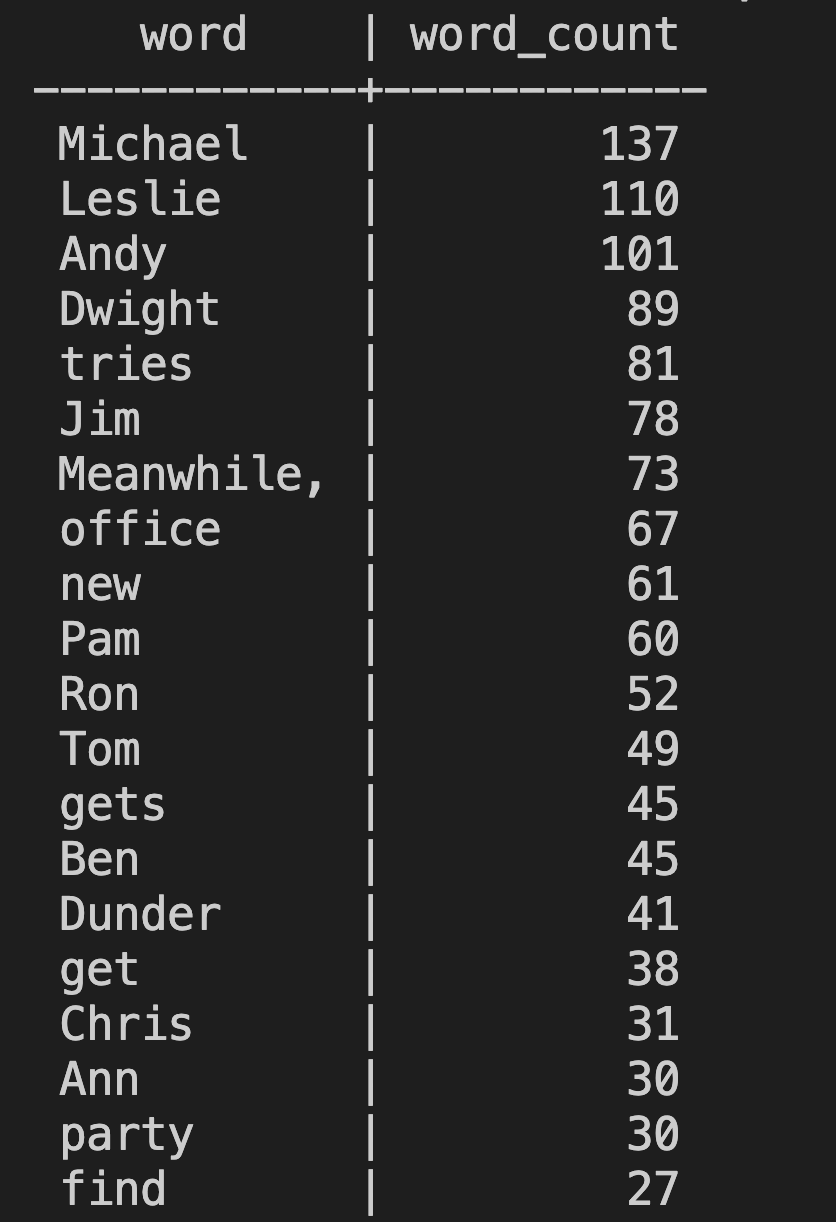
\includegraphics[width=.3\textwidth]{q1.png}
    \end{center}

\clearpage
    \item What are the top five contributing writers across both shows in terms of total episodes written, and what are their average ratings and viewership for the episodes they wrote for each show?

    \begin{minted}[breaklines]{sql}
SELECT
    ew.name,
    COUNT(*) AS total_episodes_written,
    COUNT(CASE WHEN ew.episode_show = 'The Office' THEN 1 END) AS office_episodes,
    ROUND(AVG(CASE WHEN ew.episode_show = 'The Office' THEN e.rating END), 3) AS office_avg_rating,
    ROUND(AVG(CASE WHEN ew.episode_show = 'The Office' THEN e.us_viewers END), 3) AS office_avg_views,
    COUNT(CASE WHEN ew.episode_show = 'Parks and Recreation' THEN 1 END) AS parks_episodes,
    ROUND(AVG(CASE WHEN ew.episode_show = 'Parks and Recreation' THEN e.rating END), 3) AS parks_avg_rating,
    ROUND(AVG(CASE WHEN ew.episode_show = 'Parks and Recreation' THEN e.us_viewers END), 3) AS parks_avg_views
FROM
    episode_writer ew
JOIN
    episode e ON ew.episode_show = e.show 
        AND ew.episode_season = e.season 
        AND ew.episode_episode_in_season = e.episode_in_season
GROUP BY
    ew.name
ORDER BY
    total_episodes_written DESC
LIMIT 5
    \end{minted}


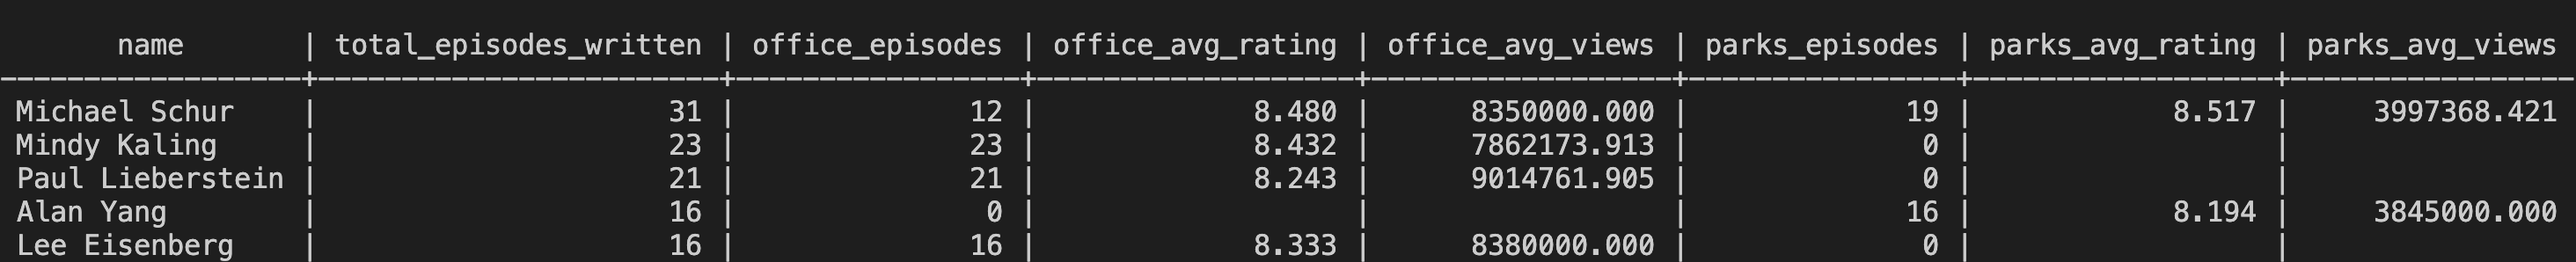
\includegraphics[width=1\textwidth]{q2.png}

\item For those who directed both shows, which show outperformed the other for the episodes they directed? 
    \begin{minted}[breaklines]{sql}
WITH DirectorStats AS ( 
    SELECT 
        director, 
        show, 
        COUNT(DISTINCT description) AS total_episodes, 
        AVG(rating) AS average_rating 
    FROM 
        episode 
    WHERE 
        director IN ( 
            SELECT DISTINCT director 
            FROM episode 
            GROUP BY director 
            HAVING COUNT(DISTINCT show) > 1 
        ) 
    GROUP BY 
        director, show 
) 
SELECT 
    ds.director, 
    SUM(ds.total_episodes) AS total_episodes, 
    SUM(CASE WHEN ds.show = 'Parks and Recreation' THEN ds.total_episodes ELSE 0 END) AS parks_episodes, 
    AVG(CASE WHEN ds.show = 'Parks and Recreation' THEN ds.average_rating END) AS parks_avg_rating, 
    SUM(CASE WHEN ds.show = 'The Office' THEN ds.total_episodes ELSE 0 END) AS office_episodes, 
    AVG(CASE WHEN ds.show = 'The Office' THEN ds.average_rating END) AS office_avg_rating, 
    CASE WHEN MAX(CASE WHEN ds.show = 'Parks and Recreation' THEN ds.average_rating END) > 
                  MAX(CASE WHEN ds.show = 'The Office' THEN ds.average_rating END) 
         THEN 'Parks and Recreation' 
         ELSE 'The Office' 
    END AS higher_rated_show 
FROM 
    DirectorStats ds 
GROUP BY 
    ds.director 
ORDER BY 
    total_episodes DESC; 

    \end{minted}

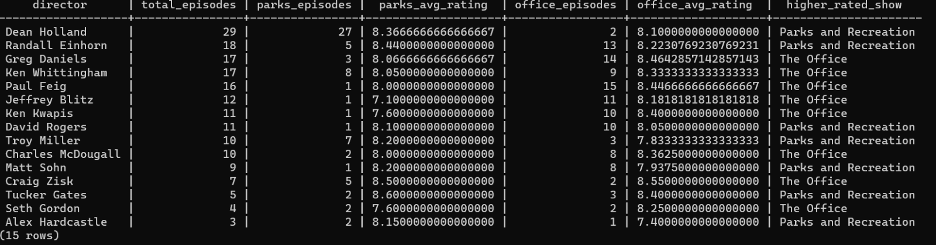
\includegraphics[width=1\textwidth]{q3.png}

 \end{enumerate}

\section*{\underline{What performance improvements did you make to your schema?}}
yes

\clearpage
\section*{\underline{Visualizing the Data}}

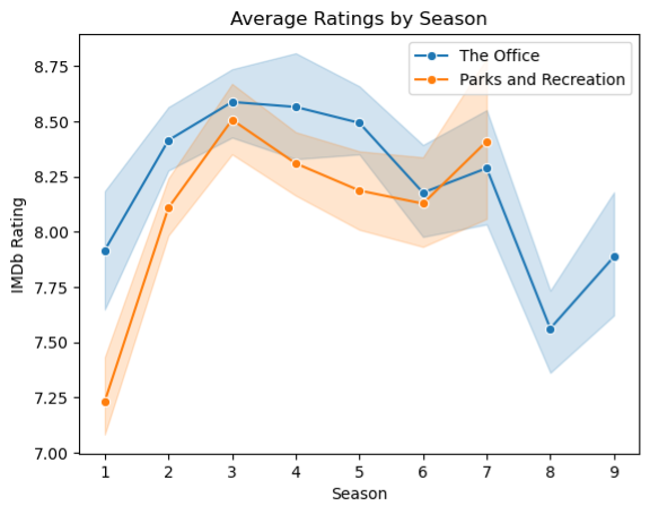
\includegraphics[width=0.6\textwidth]{avgRating.png}
\\
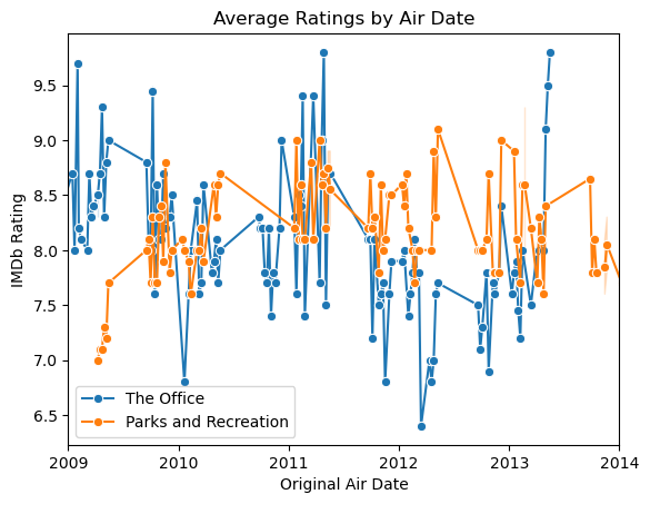
\includegraphics[width=0.6\textwidth]{avgRatingbyAir.png}
\\
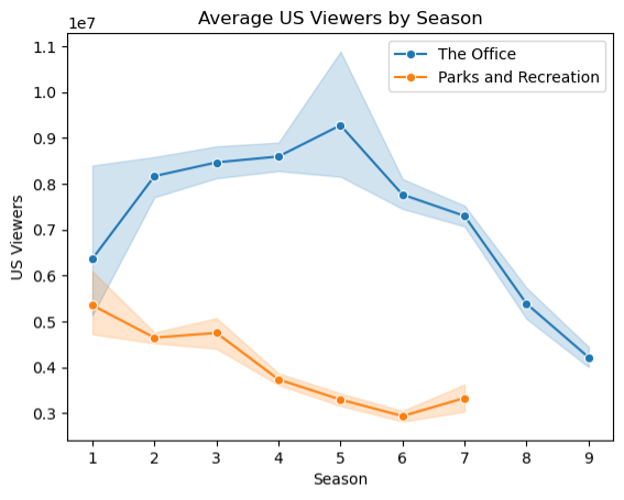
\includegraphics[width=0.6\textwidth]{avgViewerSeason.png}


\section*{\underline{Technical challenges in obtaining, manipulating, and loading the dataset(s)}}
When loading our data, we douns

% Rest of your document

\end{document}
